\section{Extruding PLCL\label{methodology:extrudingPLCL}}

\subsection{Summary of PLCL Extrusions\label{methodology:extrudingPLCL:plclSummary}}

A significant portion of the research in this thesis pertains to extruding PLCL into a 3D printable filament. Multiple methods were employed to eventually achieve this. In summary, powder extrusions were first attempted. This was followed by manually and then automatically combining PLA and PCL pellets in a single screw extruder. Two extruders, 3Devo Filament Maker 1 and the Felfil Evo, were used to conduct these extrusions. Finally, shredding or regrinding the initial PLCL output and re-extruding was tested to address thickness tolerance concerns. Figure~\ref{methodology:extrudingPLCL:plclSummary} outlines this process at a high level.

\begin{figure}[h!]
        \centering
        \includegraphics[width=\linewidth]{../figs/methodology/plclExtrusions/plcl_extrusion_summary.png}
        \caption{Overview of the progression of PLCL extruding research.}
        \label{fig:methodology:extrudingPLCL:plclSummary}
\end{figure}

Additionally,~\fullref{tab:appendix:extrusionSummary} details all extrusions performed and their results.

\subsection{Powder Extrusions\label{sec:methodology:extrudingPLCL:powderExtrusion}}

Based on material availability, the team attempted to extrude PLCL powder to create PLCL filament. While pellets are more commonly extruded than powders (see~\fullref{sec:literatureReview:extrusion:powder}), the team was unable to source PLCL pellets at a scalable price. As a result, Nomisma PLCL powder was used~\cite{RefWorks:RefID:387-nomisma} for these initial extrusions on a 3Devo Filament Maker 1 single screw extruder.

Prior to extruding, the PLCL powder was dried in a vaccuum oven at 45\textcelsius ~overnight based on the material manufacturer's recommendations. The Polymer Synthesis Research Facility (PSRF) at Ohio State University was utilized for this task (see~\fullref{sec:methodology:externalLabs:polymersLab} for more information on research conducted with this additional lab).

The powder was measured and poured into the extruder as shown in Figure~\ref{fig:methodology:extrudingPLCL:powderExtrusion}.

\begin{figure}[h!]
        \centering
        \includegraphics[width=0.7\linewidth]{../figs/methodology/plclExtrusions/powderExtrusion/powder_extrusion.png}
        \caption{Performing PLCL powder extrusion. Measuring powder (left) and pouring into extruder (right).}
        \label{fig:methodology:extrudingPLCL:powderExtrusion}
\end{figure}

In addition to pouring the powder, a pusher inspired by the Devostick was employed~\cite{RefWorks:RefID:396-3devotroubleshooting}. This is a rectangular piece of wood used to compress the material in hopes of resolving feeding issues. Using the pusher piece is shown below in ~\autoref{fig:methodology:extrudingPLCL:devostick}.

\begin{figure}[h!]
        \centering
        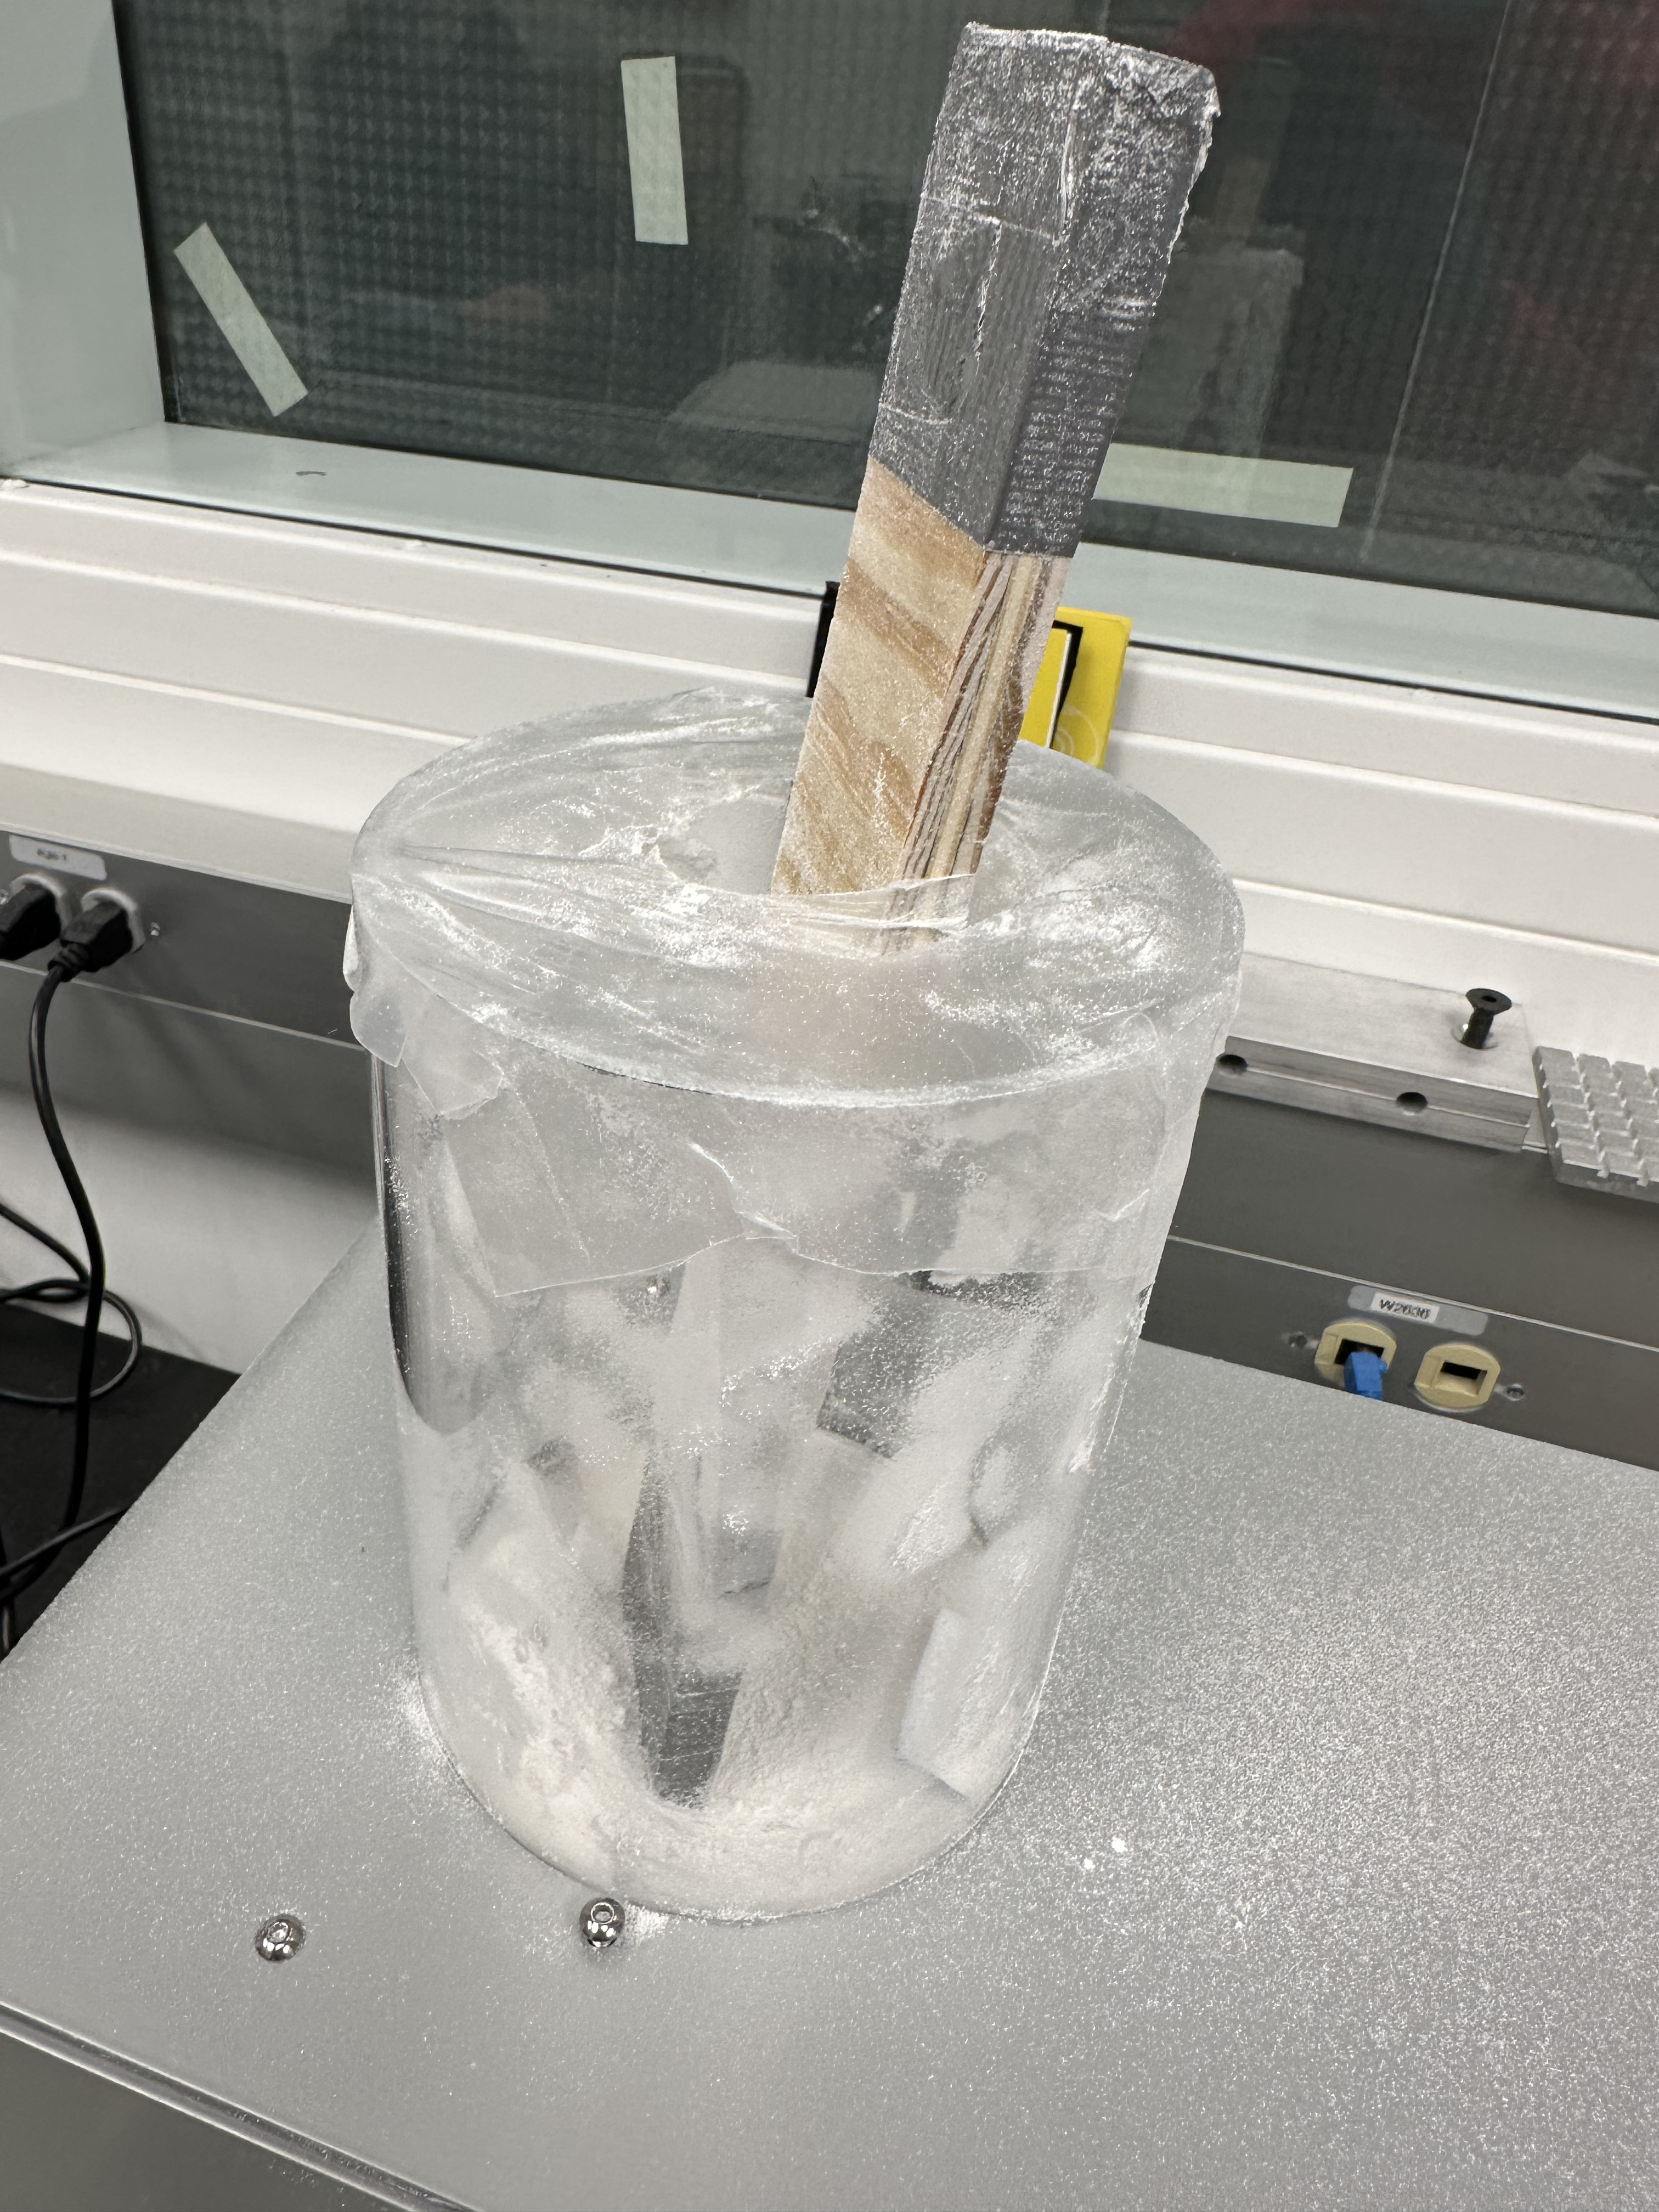
\includegraphics[width=0.5\linewidth]{../figs/methodology/plclExtrusions/powderExtrusion/devostick.png}
        \caption{Using the self-made "Devostick".}
        \label{fig:methodology:extrudingPLCL:devostick}
\end{figure}

This extruder has four heat zones with heater 4 (H4) being closest to the hopper and heater 1 (H1) being closest to the nozzle. Heaters 4 through 1 were set to 205\textcelsius, 200\textcelsius, 195\textcelsius, and 190\textcelsius ~respectively based on 3Devo customer support recommendations. The RPM for the extruder was set to 3.5.

To achieve these temperatures, the extruder was first run at PLA presets (H4-H1: 170, 185, 190, 170 (all in \textcelsius)). Temperatures were raised to HDPE presets (190\textcelsius ~across all heat zones) and HDPE was introduced into the extruder. Finally, temperatures were raised to the PLCL extruding temperatures and the PLCL powder was introduced into the extruder. DevoVision was used to monitor extruder parameters and variables such as current and heater temperatures.

The results and discussion for this experiment can be found in~\fullref{sec:results:extrudingPLCL:powderExtrusion} and~\fullref{sec:discussion:extrudingPLCL:powderExtrusion} respectively.

\subsection{Pellet Extrusions\label{sec:methodology:extrudingPLCL:pelletExtrusions}}
% Pivoted to pellets based on powder struggles and lit review
Based on the  difficulties and inherent brittleness of powder-based extrusions, the team explored relevant literature and decided to combine the copolymers of PLCL, PLA and PCL, in pellet form. This allows the extrusion to be completed with pellets rather than powder(s).

\subsubsection{Combining Raw Materials\label{sec:methodology:extrudingPLCL:pelletExtrusions:combiningMaterials}}
After deciding to explore pellet-based extrusions using PLA and PCL pellets, the team investigated how to best combine the two materials into a semi-homogenous mixture for extruding. Various methods the team explored were utilizing equipment with the College of Pharmacy, injection molding, chemically combining the two materials, mixing the materials in a tumbler, and discussing mixing concerns with extrusion subject-matter experts (SMEs) in the Department of Industrial Systems and Engineering at Ohio State University.~\fullref{sec:discussion:extrudingPLCL:pelletExtrusions:combiningMaterials} explains the findings of this investigation.

See~\fullref{sec:literatureReview:PLCL} for relevant literature on synthesizing PLCL.

\paragraph*{College of Pharmacy}
The team contacted the college of pharmacy at The Ohio State University due to the substantial mixing that occurs in pharmaceutical research. The team also toured the college of pharmacy's research facilities to better understand their equipment capabilities.

\paragraph*{Injection Molding}
The team also explored injection molding as a means of combining the PLA and PCL pellets. This was done by reviewing relevant literature and meeting with knowledgable professors at Ohio State University.

\paragraph*{Chemically Combining Materials}
Following existing literature, the team explored chemically combining PLA and PCL such as by dissolving the materials in dichloromethane (DCM) or chloroform.

The team also evaluated melting the pellets together on a hotplate with a magnetic and manual stirrer as shown below in~\autoref{fig:methodology:extrudingPLCL:meltingOnHotplate}

\begin{figure}[h!]
        \centering
        \includegraphics[width=0.5\linewidth]{../figs/methodology/plclExtrusions/pelletExtrusions/combining_on_hotplate.png}
        \caption{Melting PLA and PCL using a hotplate with mixing (left) and final output (right).}
        \label{fig:methodology:extrudingPLCL:meltingOnHotplate}
\end{figure}

\paragraph*{3D Printable Mixing Systems}

Mixing the pellets in a tumbler styler mixer was also explored. To lower the cost and development time, 3D printing a mixing system was explored. Various premade models of rotary tumbler mixers were found through online CAD repositories such as Thingiverse. Examples of 3D printable mixers are shown in Figure~\ref{fig:methodology:extrudingPLCL:3dPrintableMixers}

\begin{figure}[h!]
        \centering
        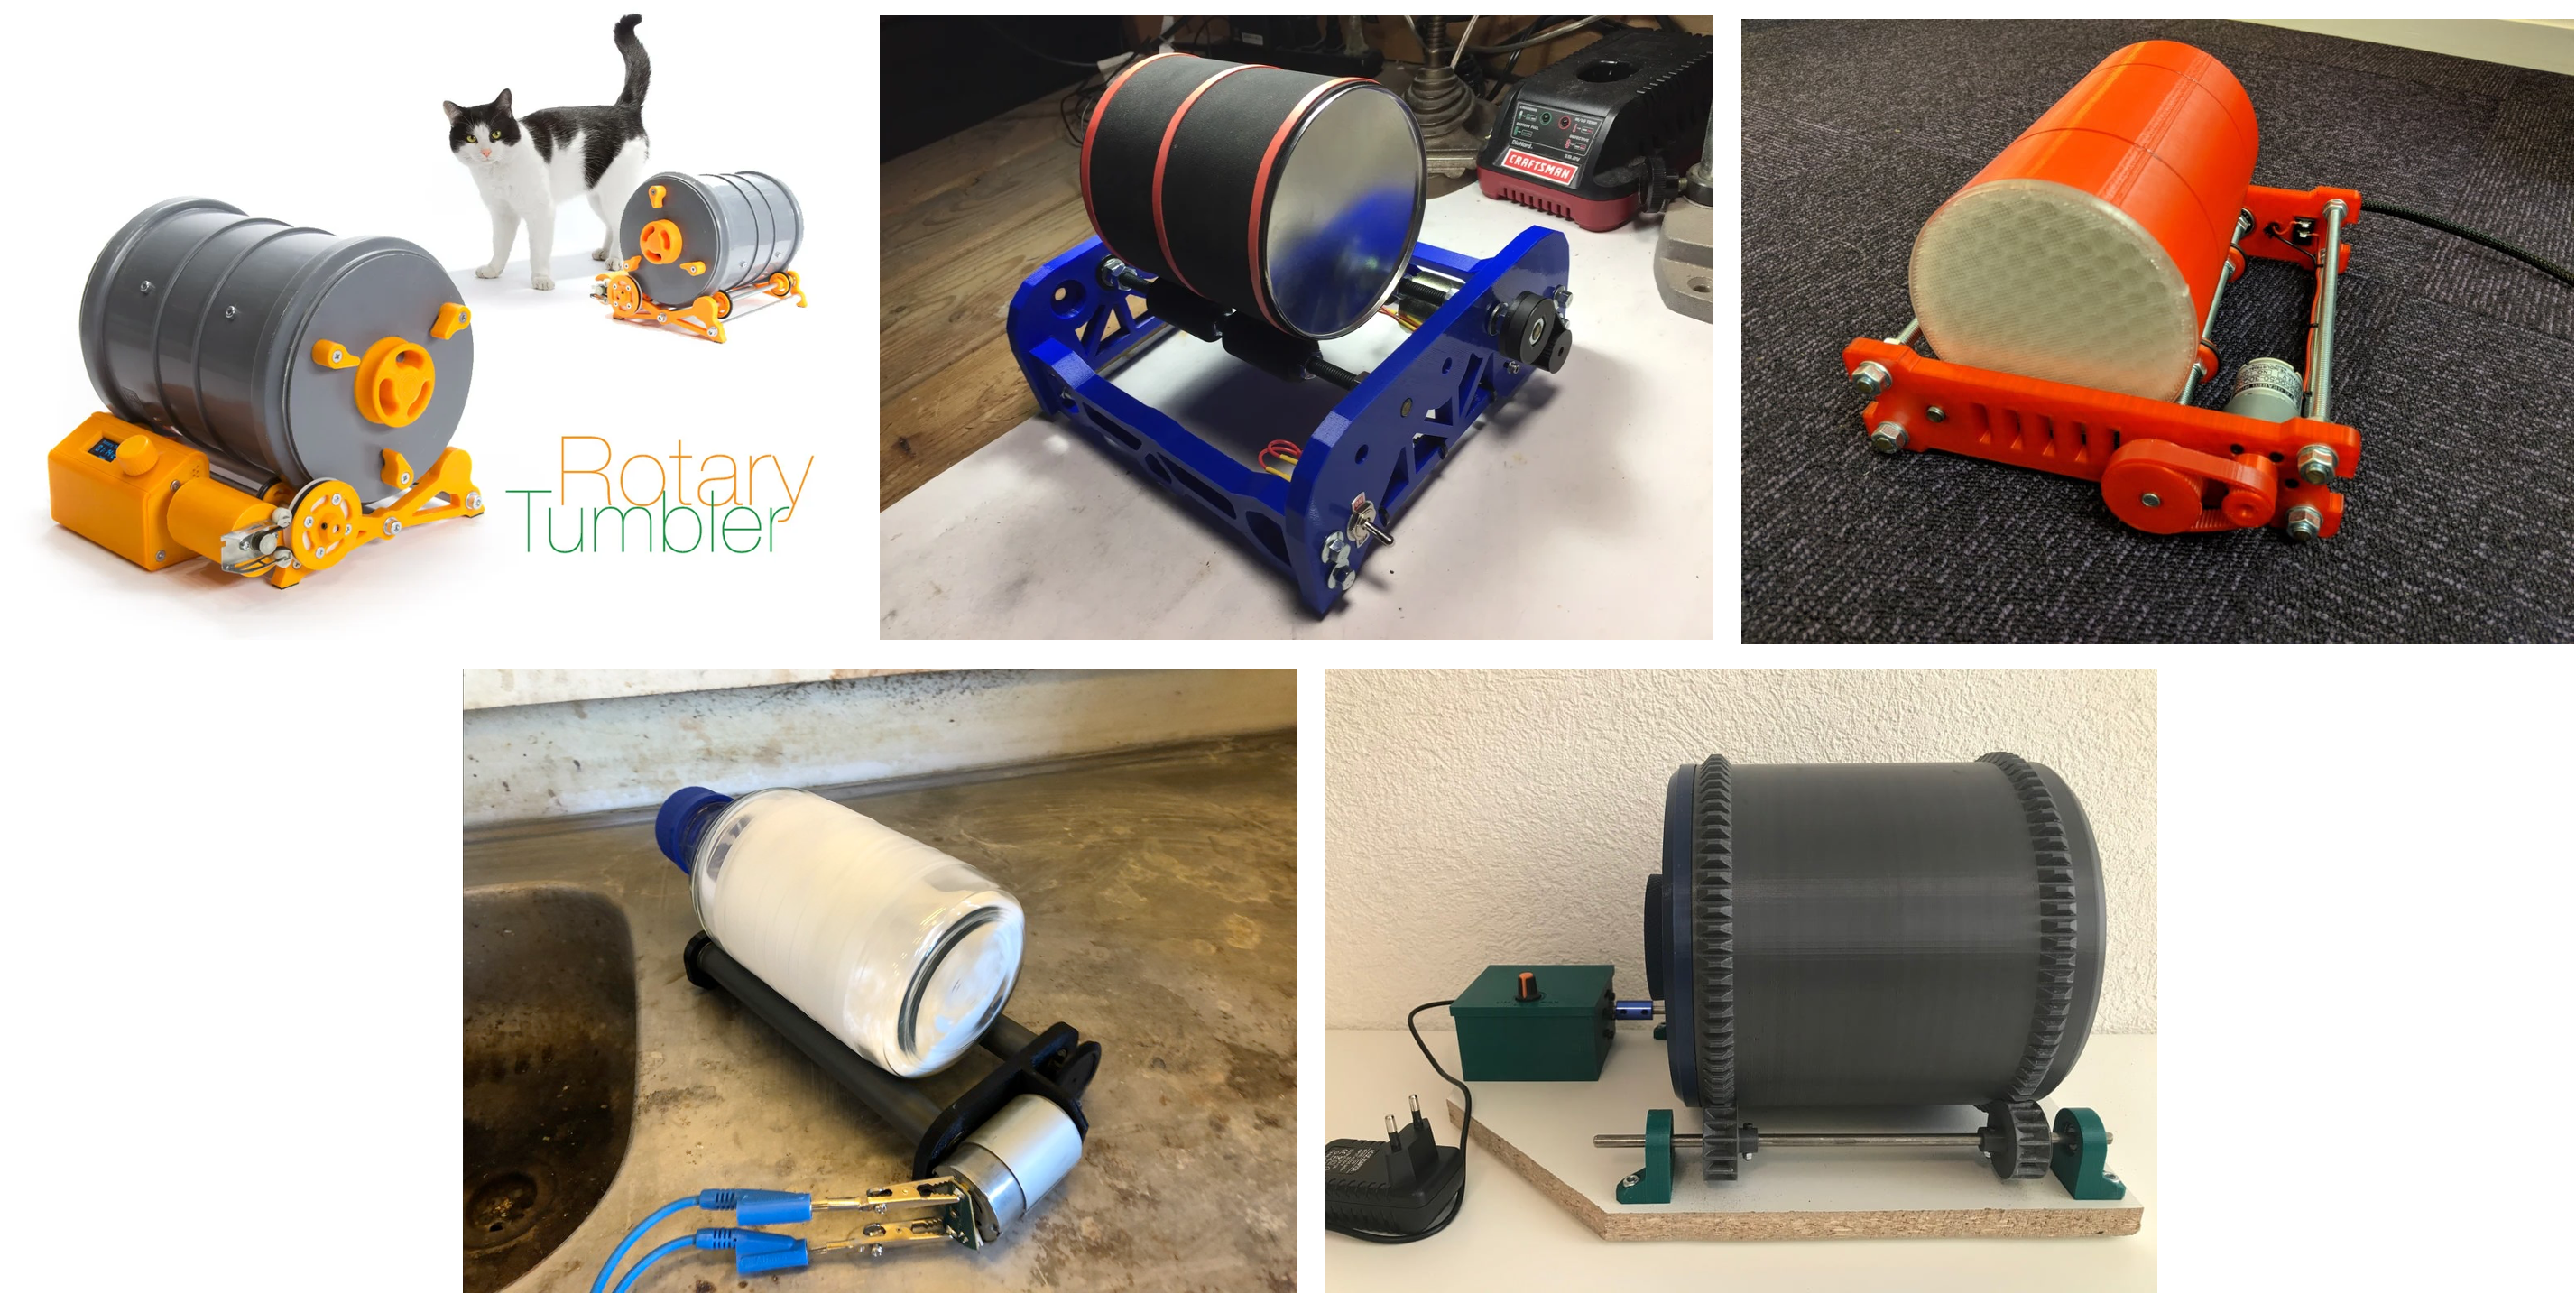
\includegraphics[width=0.7\linewidth]{../figs/methodology/plclExtrusions/pelletExtrusions/3d_printed_mixers.png}
        \caption{Various 3D printable tumbler mixers~\cite{RefWorks:RefID:482-lucasfrit2021ball,RefWorks:RefID:483-bluepop42017rock,RefWorks:RefID:484-dariocarioli2018rotary,RefWorks:RefID:485-jonathanlundstrom2018simple,RefWorks:RefID:486-perinski2018rotary}.}
        \label{fig:methodology:extrudingPLCL:3dPrintableMixers}
\end{figure}

\paragraph*{Discussions with ISE Department}
The team also met with extrusion subject-matter experts in the Industrial and Systems Engineering (ISE) department at The Ohio State University. This included Dr. Rachmat Mulyana.

\subsection{Initial Pellet Extrusion\label{sec:methodology:extrudingPLCL:pelletExtrusions:initialExtrusion}}

PLA pellets were purchased from 3DXTECH and PCL pellets were ordered from Sigma Aldrich~\cite{RefWorks:RefID:487-ecomax,RefWorks:RefID:488-polycaprolactone}. Following manufacturer recommendations, PLA and PCL pellets were dried overnight in a vacuum oven at 55\textcelsius and 40\textcelsius respectively prior to extruding.

After deciding to combine PLA and PCL pellets manually in a jar (see~\fullref{sec:discussion:extrudingPLCL:pelletExtrusions:combiningMaterials}), an initial pellet extrusion was performed.

Figure~\ref{fig:methodology:extrudingPLCL:mixingPellets} shows the pellet mixture before and after mixing. The white colored pellets are PCL and the tan colored pellets are PLA. A 70/30 mixture of PLA/PCL was created by weight with roughly 70g of PLA and 30g of PCL.

\begin{figure}[h!]
        \centering
        \includegraphics[width=0.7\linewidth]{../figs/methodology/plclExtrusions/pelletExtrusions/mixing_pellets_manually.png}
        \caption{Mixing pellets manually. Unmixed (left), mixed (middle and right).}
        \label{fig:methodology:extrudingPLCL:mixingPellets}
\end{figure}

In this extrusion, the 3Devo Feeder was used for the first time. The temperature profile was is shown below in Table~\ref{tab:methodology:extrudingPLCL:initialPelletExtrusion:tempPresets} based on existing literature~\cite{RefWorks:RefID:253-åkerlund2022effect}. All pellets were poured into the hopper with the Feeder running and the extrusion began.

\begin{table}[h!]
        \centering
        \caption{Initial pellet extrusion temperature presets\label{tab:methodology:extrudingPLCL:initialPelletExtrusion:tempPresets}}
        \begin{tabular}{l c}
                \hline
                \textbf{Heater} & \textbf{Temperature (\textcelsius)} \\
                \hline
                H4              & 140                                 \\
                H3              & 155                                 \\
                H2              & 160                                 \\
                H1              & 160                                 \\
                \hline
        \end{tabular}
\end{table}

Results and discussion of this extrusion can be found in ~\fullref{sec:results:extrudingPLCL:pelletExtrusions:initialPelletExtrusion} and ~\fullref{sec:discussion:extrudingPLCL:pelletExtrusions:initialPelletExtrusion} respectively.

\subsection{PCL Temperature Study\label{sec:methodology:extrudingPLCL:pelletExtrusions:pclExtrusions}}
% Extruded just PCL to find extrudable temp and make sure it overlapped with PLA
% Found starve feeding helps with melting in the hopper
% Inspired to develop automatic starve feeder

Based on findings from the initial pellet extrusion (see~\fullref{sec:discussion:extrudingPLCL:pelletExtrusions:initialPelletExtrusion}), a study was performed to determine the working extrusion temperature of PCL pellets. A PCL extrusion process developed by 3Devo was followed which first involved  extruding PLA pellets at normal presets. All heaters were then set to 170\textcelsius ~and PCL was introduced. Once the filament output had shifted from PLA to PCL, which is apparent based on the filament color being white rather than clear, the temperature of all heaters was lowered to 60\textcelsius. From here, the temperature was raised in increments of 10\textcelsius ~to determine how high of a temperature PCL could be easily extruded at~\cite{RefWorks:RefID:489-3devo2024extrusion}.

Based on time available, this extrusion was divided into two sequential extrusions. The first tested PCL between 60\textcelsius ~and 110\textcelsius ~while the second extrusion tested PCL between 120\textcelsius ~and 180\textcelsius.

Starve feeding was also explored during these extrusions. Extrusion 1 (60-110\textcelsius) employed manual starve feeding. An Excel spreadsheet was used to track the amount of PCL poured and the time between pours. A section of that spreadsheet is shown below in Figure~\ref{fig:methodology:extrudingPLCL:manualStarveFeedingLog}.

\begin{figure}[h!]
        \centering
        \includegraphics[width=\linewidth]{../figs/methodology/plclExtrusions/pelletExtrusions/manual_starve_feeding_log.png}
        \caption{Section of manual starve feeding Excel spreadsheet.}
        \label{fig:methodology:extrudingPLCL:manualStarveFeedingLog}
\end{figure}

Results and discussion of the PCL temperature study can be found in ~\fullref{sec:results:extrudingPLCL:pelletExtrusions:pclTempStudy} and ~\fullref{sec:discussion:extrudingPLCL:pelletExtrusions:pclTempStudy} respectively. Results and discussion of the manual starve feeding can be found in ~\fullref{sec:results:extrudingPLCL:pelletExtrusions:manualStarveFeeding} and ~\fullref{sec:discussion:extrudingPLCL:pelletExtrusions:manualStarveFeeding} respectively.

\subsection{Starve Feeding Based Pellet Extrusions\label{sec:methodology:extrudingPLCL:pelletExtrusions:usingStarveFeeder}}
% Finally successful but too thin
% Shredding and re-extruding looked promising (using extruder to combine pellets initially) but still led to variable flow rate due to regrind
Based on the repetitive and exact nature of the manual starve feeding, an automatic starve feeder was developed (see ~\fullref{sec:discussion:extrudingPLCL:pelletExtrusions:manualStarveFeeding} for more details on this decision). This development is detailed in ~\fullref{sec:methodology:starveFeeder}.

The starve feeder was first tested on PCL during the second temperature test extrusion from 120\textcelsius ~to 180\textcelsius. Once it was proven to work, the starve feeder was used on a PLCL extrusion.

\subsubsection{PLCL Extrusion with Starve Feeder\label{sec:methodology:extrudingPLCL:pelletExtrusions:usingStarveFeeder:PLCLExtrusion}}
% Worked but too thin

\subsection{Felfil System\label{sec:methodology:extrudingPLCL:felfilSystem}}

\subsubsection{Felfil Evo Initial Testing\label{sec:methodology:extrudingPLCL:felfilSystem:felfilEvo}}

\paragraph*{Initial Repairs\label{sec:methodology:extrudingPLCL:felfilSystem:felfilEvo:initialRepairs}}
% a. Tried replacing the hopper without fully disassembling
% b. Led to the barrel not being secured and spinning out of place
% c. Disassembled fully, cleaned, and reassembled correctly
% d. Replaced broken O-ring in nozzle

\paragraph*{Initial PLA Testing\label{sec:methodology:extrudingPLCL:felfilSystem:felfilEvo:initialTesting}}
% a. Tested with PLA pellets which worked wonderfully

\paragraph*{Learnings from Initial Testing\label{sec:methodology:extrudingPLCL:felfilSystem:felfilEvo:learningsFromInitialTesting}}
% a. Pellets remain the best material to extrude with
% b. Even though we couldn't get the system to work with powders, it can likely work well with pellets
\subsubsection{Felfil Evo PLCL Extrusion\label{sec:methodology:extrudingPLCL:felfilSystem:felfilEvoPLCL}}

\paragraph*{Initial PLCL Extrusion Attempts\label{sec:methodology:extrudingPLCL:felfilSystem:felfilEvoPLCL:initialAttempts}}
% a. Can extrude PLCL at proper thickness on 1st pass and faster than 3Devo
% b. First time we've had successul proper thickness PLCL filament

\paragraph*{Clumping at Hopper\label{sec:methodology:extrudingPLCL:felfilSystem:felfilEvoPLCL:clumpingAtHopper}}
% a. Noticed clumping at hopper due to metal wall closest to barrel
% b. Tried using starve feeding method but would need refining/testing
% c. Planned to look into isolating that metal wall section from the raw materials

\subsubsection{Felfil Evo Hopper Improvements\label{sec:methodology:extrudingPLCL:felfilSystem:felfilEvoHopperImprovements}}

\paragraph*{Silicone Coating\label{sec:methodology:extrudingPLCL:felfilSystem:felfilEvoHopperImprovements:siliconeCoating}}
% a. Looked into silicone with adhesive backing to block the heat (like what's used in Rasbperry Pi)
% b. Talked with Chris in electronics lab to see if he's run across that ever
% c. Initial google search on available materials

\paragraph*{3D Printed Hopper Insert\label{sec:methodology:extrudingPLCL:felfilSystem:felfilEvoHopperImprovements:3dPrintedHopperInsert}}
% a. Created a 3D printed insert to block the heat transfer
% b. Modeled it in SolidWorks after using the existing CAD files to create an assembly of the hopper
% c. Took 5 versions to properly account for the screw (couldn't measure by hand without fully disassembling machine)
% d. Added thickness and slope to address thin insert still getting hot
% i. Add distance between wall and raw materials

\subsubsection{Felfil Spooler+\label{sec:methodology:extrudingPLCL:felfilSystem:felfilSpooler}}

\paragraph*{Noticed Need to Log Thickness\label{sec:methodology:extrudingPLCL:felfilSystem:felfilSpooler:noticedNeedToLogThickness}}
% a. Realized I needed to log thickness data to analyze it like DevoVision does

\paragraph*{Accessing Firmware\label{sec:methodology:extrudingPLCL:felfilSystem:felfilSpooler:accessingFirmware}}
% a. Felfil is open source and run on an Arduino Nano
% b. I was able to access the current firmware (V1.8) and modify it
% c. USB-MiniB port is accessible through side of spooler or by taking casing off

\paragraph*{Modifying Firmware\label{sec:methodology:extrudingPLCL:felfilSystem:felfilSpooler:modifyingFirmware}}
% a. I looked through the firmware and found where the live diameter reading was stored
% b. Started by printing to serial monitor
% c. Created python script to store readings in a csv for easy logging and graphical analysis

\subsubsection{Felfil Shredder\label{sec:methodology:extrudingPLCL:felfilSystem:felfilShredder}}
% a. Started by shredding multiple times until regrind size looked uniform
% b. Downloaded sieve from Felfil to control for size and make sure everything is ~5mm x 5mm
% c. Discovered that medium-thick filament shreds best

\subsection{Purging Compounds\label{sec:methodology:extrudingPLCL:purgingCompounds}}
\hl{Exploration of purging compounds to find DP-K works best}
% iii.	Purging Compounds
% 1.	Found initial supplier of 3Devo DevoClean Mid-Temp
% 2.	Worked with supplier (Dyna-Purge) to find ideal purging material
% a.	Tried L then D2 (needs HDPE) then K

\subsubsection{Initial Purging Process\label{sec:methodology:extrudingPLCL:purgingCompounds:initialProcess}}

\subsubsection{Supplier Discovery\label{sec:methodology:extrudingPLCL:purgingCompounds:supplierDiscovery}}

\subsubsection{Dyna-Purge Collaboration\label{sec:methodology:extrudingPLCL:purgingCompounds:dynaPurgeCollaboration}}
% Tried L then D2 (needs HDPE) then K

\subsection{PLA with Barium Sulfate\label{sec:methodology:extrudingPLCL:plaWithBaSO4}}
